\chapter{Source-bound verification of the earlier computational continuation}
The following preserved execution record refers to the pinned program-three release. This unified edition has an additional integration record; earlier test counts are not represented as expanded proof coverage.

\input{verification-summary}

The published Python tests exercise the ordinary and optimized interpreters. The formal audit prints each new declaration and its axiom inventory, rejects warnings, rejects \texttt{sorryAx}, and binds the exact source to Lean 4.24.0 and the recorded mathlib revision. The finite arithmetic module checks its entire small curve table; the general Kraus and rank-count modules verify their displayed quantified statements. The whole physical interpretation is not encoded by a successful process exit.

The browser executes the emitted reversible gates and the learned four-qubit circuit. It independently recomputes all 72 fixed sky templates and all three methods for observed maps or explicitly labeled injected profiles. Its scientific JSON assets are SHA-256 checked before use. Interactive state is exportable and URL-backed; keyboard and mobile behavior are tested. A corrupted asset is rejected rather than displayed under a successful-verification badge.

The original workstation completed genuine cuStateVec checks of both $p=7$ arithmetic circuits on a complex superposition spanning all 2,048 declared input words. The observed maximum amplitude discrepancy and dirty-ancilla probability were zero. Six trained-channel gate checks agreed with the independent Kraus implementation to $5.56\times10^{-16}$. The subsequent independent repository runner has no GPU and does not relabel those measurements as its own. The $p=13$ circuits retain exhaustive basis verification without a dense-GPU claim.

Desktop Commander reached its monthly usage limit during the continuation. No retry, reconnection, service restart, credential extraction or alternate access to the paused device was used. Independent repository CI rebuilt the source and evidence on a standard public CPU runner. Remote clone synchronization after that pause is not asserted. The original Mora-3 training campaign remains outside this task.

\begin{figure}[p]\centering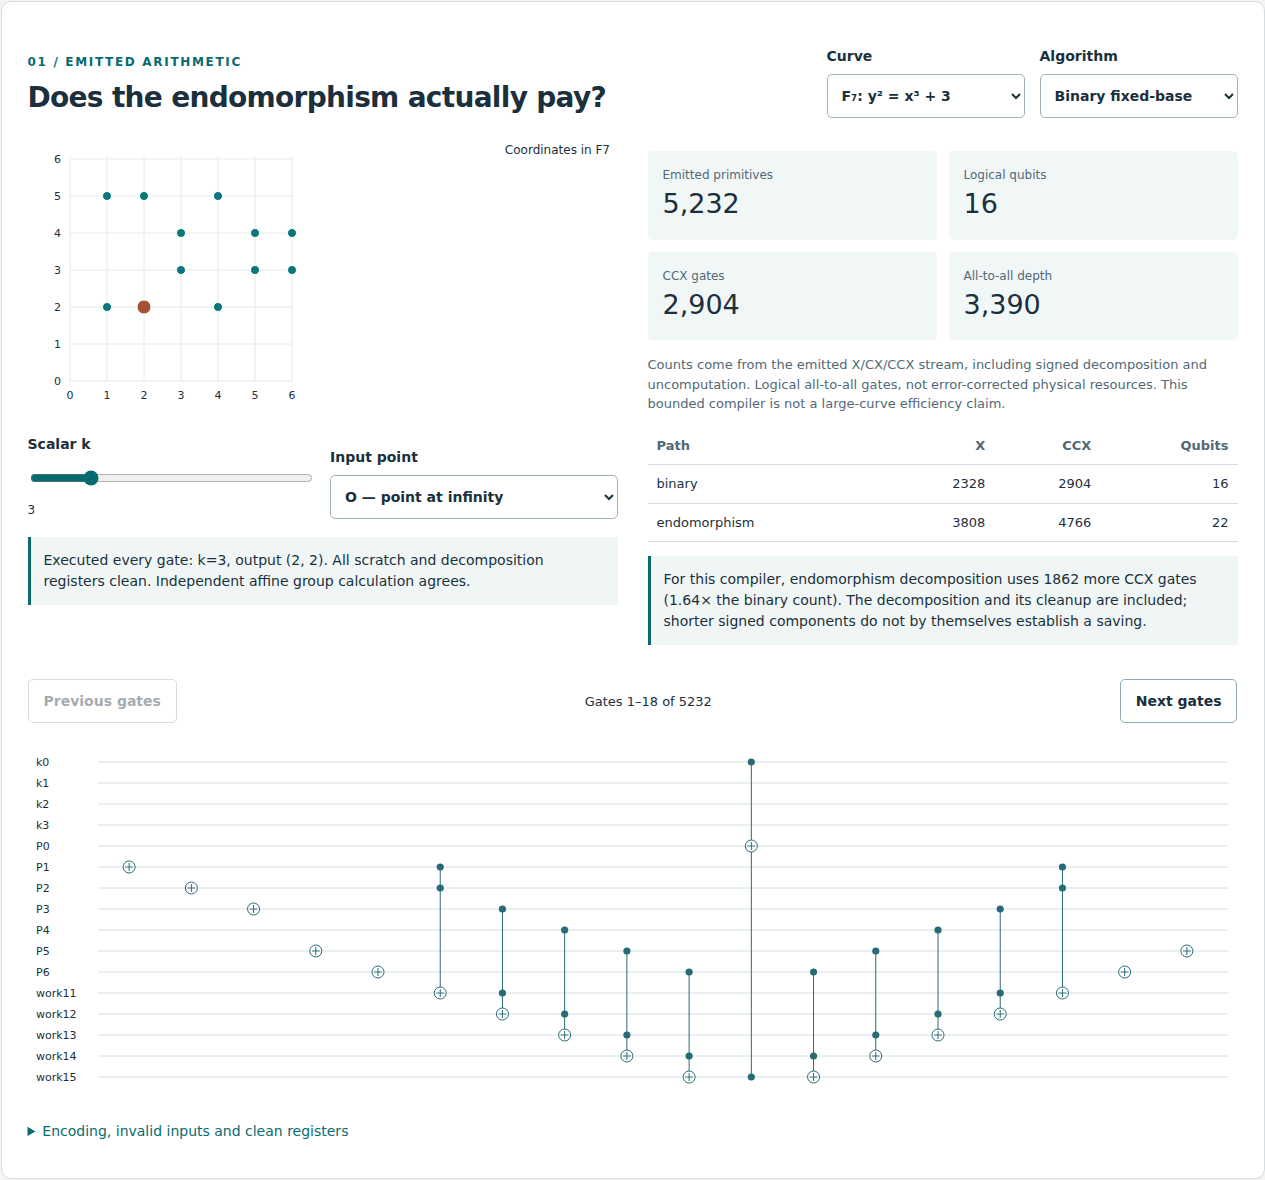
\includegraphics[width=\textwidth,height=.82\textheight,keepaspectratio]{arithmetic.png}\caption{The actual arithmetic explorer: finite-field points, complete emitted-gate counts, invalid-word behavior and a paginated circuit stream.}\end{figure}
\begin{figure}[p]\centering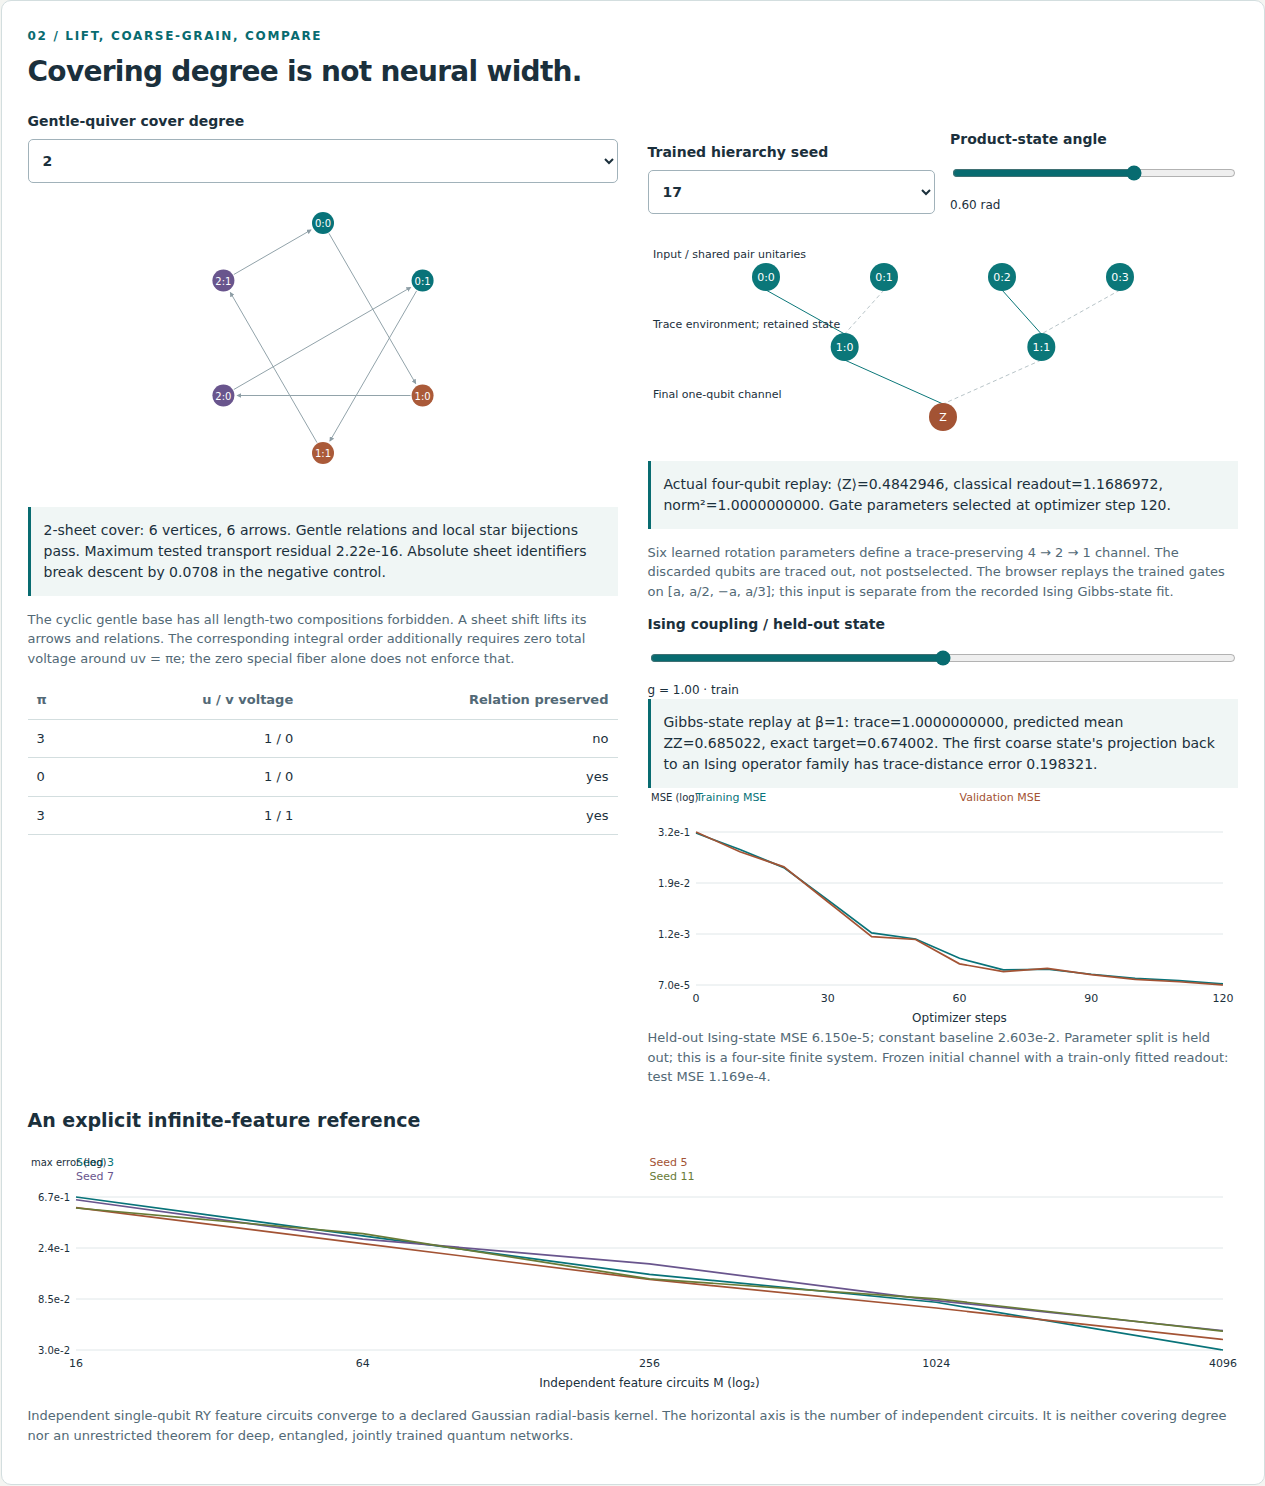
\includegraphics[width=\textwidth,height=.82\textheight,keepaspectratio]{coverings.png}\caption{Voltage covers, learned hierarchical channels, effective-Hamiltonian error and the separately scaled independent-feature width experiment.}\end{figure}
\begin{figure}[p]\centering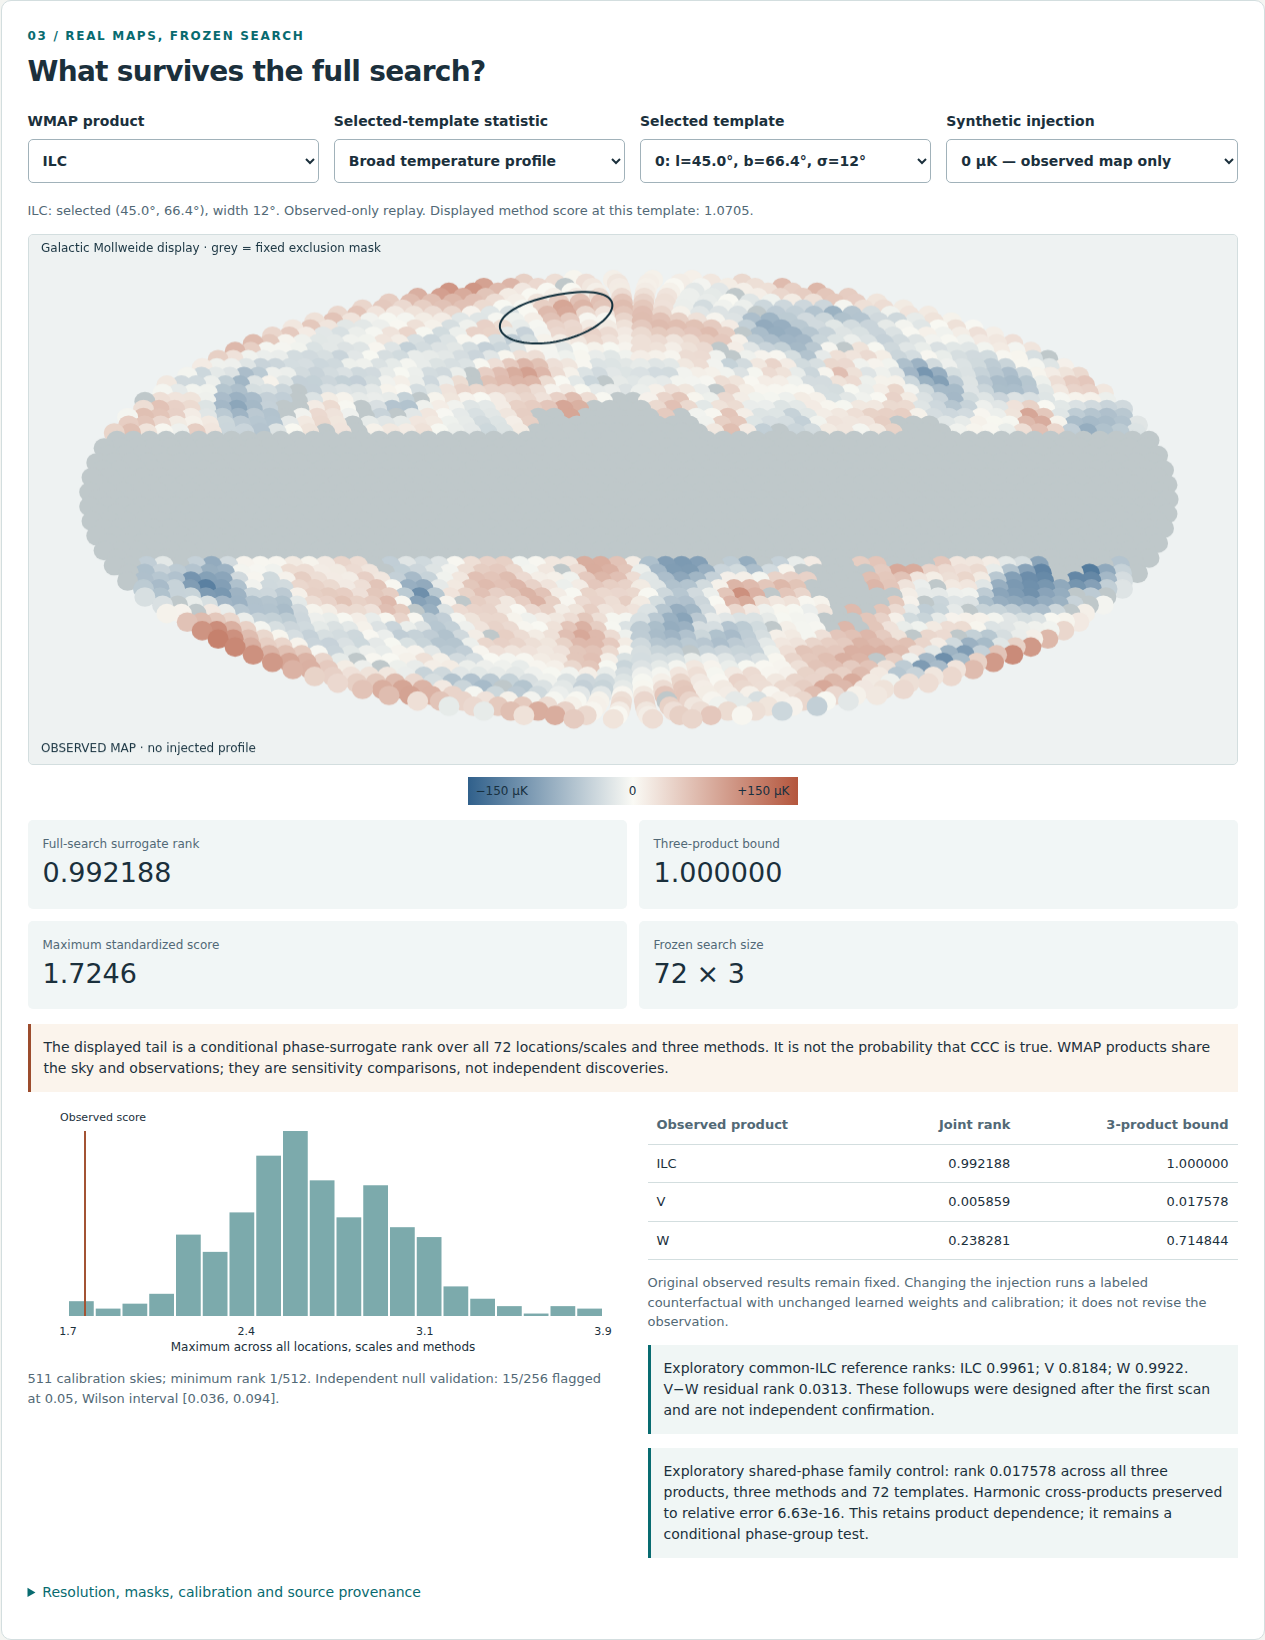
\includegraphics[width=\textwidth,height=.82\textheight,keepaspectratio]{sky.png}\caption{Observed WMAP maps and a complete frozen search. Synthetic injections and post-inspection sensitivity tests are explicitly distinguished from the original observations.}\end{figure}
